




\section{
	Procesos estocásticos
}

\subsection{Definición} Un \textbf{proceso estocástico }$\lbrace X_t, t \in T \rbrace$ es una colección de variables aleatorias definidas sobre el mismo espacio de probabilidad ($\Omega,S,P$). El conjunto $T$ se llama índice del proceso. Si $T$ es numerable diremos que el proceso estocástico es de tiempo discreto ($T=\lbrace 0,1,2,... \rbrace$) y si es continuo diremos que estamos ante un proceso estocástico de tiempo continuo ($T=\lbrace t, t\geq 0 \rbrace$).

\subsection{Cadena de Markov}\


Sea $\lbrace X_n, n=0,1,2,...\rbrace$ un proceso estocástico de tiempo discreto. Suponemos que en cualquier instante, el proceso toma un número finito o numerable de valores (llamados estados del proceso).
Un proceso estocástico de tiempo discreto es una \textbf{Cadena de Markov}, si para $t$=0,1,2,... y los estados $i_0, i_1,...,i_{n-1},i,j$:

$$
P(X_{n+1}=j|X_n=i, X_{n-1}=i_{n-1},...,X_1=i_1, X_0=i_0)=P(X_{n+1}=j|X_n=i_n)=p_{ij}
$$

donde $X_n=i_n$ representa que en el instante $n$ el proceso se encuentra en el estado $i_n$ y $p_{ij}\geq 0$ la probabilidad de que el proceso pase al estado $j$ cuando se encuentra en el estado $i$.

La matriz de probabilidades de transición en un paso es:


$$P=
\left(
\begin{array}{cccc}
p_{11} & p_{12} & \cdots & p_{1s} \\
p_{21} & p_{22} & \cdots & p_{2s} \\
\vdots & \vdots & & \vdots \\
p_{s1} & p_{s2} & \cdots & p_{ss} \\
\end{array}
\right)
$$
con $ \sum_{j=1}^{s} P(X_{n+1}=j|X_n=i_n)=\sum_{j=1}^{s} p_{ij}=1 $ para $i$=1,2...\\

\textbf{Nota}: Aunque la matriz de probabilidades de transición de un proceso estocástico no tiene por qué ser cuadrada, nos será útil que tenga ésta propiedad para definir probabilidades de transición en la $n$-ésima etapa.\\

\textbf{Ejemplo}:

Sea la matriz de probabilidades en un paso:

$$P=
\left(
\begin{array}{ccc}
1/3 & 1/3 & 1/3 \\
1/3 & 0 & 2/3 \\
1/2 & 1/2 & 0 \\
\end{array}
\right)
$$

Su grafo de estados es:

\begin{figure*}[h]
	\centering
	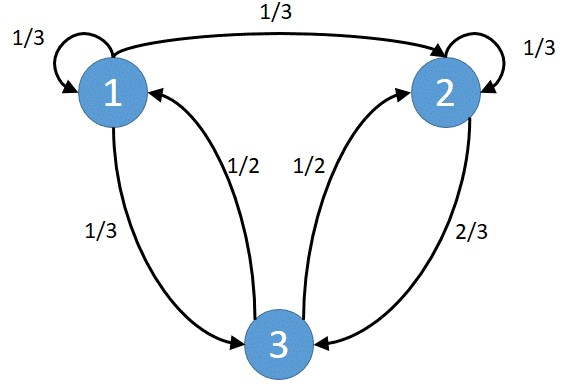
\includegraphics[width=0.4\textwidth]{grafo1}
	\label{grf1}
\end{figure*}



\subsection{Probabilidades de transición en la $\textbf{\textsl{n}}$-ésima etapa}

Supongamos que una cadena de Markov, en el instante $m$ está en el estado $i$, ¿Cuál es la probabilidad de estar en el estado $j$ después de n periodos? Esta probabilidad es independiente de $m$, así que la podemos escribir como:

$$
P(X_{m+n}=j|X_m)=P(X_n=j|X_0=i)=p_{ij}^n
$$

donde $p_{ij}^n$ se llama probabilidad del $n$-ésimo paso de transición del estado $i$ al $j$ y son los $ij$-ésimos elementos de $P^n$, donde $P$ es la matriz de probabilidades en un paso de nuestra cadena de Markov.\\


\textbf{Ejemplo}:\\ 

Sea P la matriz de probabilidades de transición en un paso del ejemplo anterior. Calcula todas las probabilidades de transición en dos pasos.


$$P^2=
\left(
\begin{array}{ccc}
1/3 & 1/3 & 1/3 \\
1/3 & 0 & 2/3 \\
1/2 & 1/2 & 0 \\
\end{array}
\right)
\left(
\begin{array}{ccc}
1/3 & 1/3 & 1/3 \\
1/3 & 0 & 2/3 \\
1/2 & 1/2 & 0 \\
\end{array}
\right)
=
\left(
\begin{array}{ccc}
21/54 & 15/54 & 18/54 \\
24/54 & 24/54 & 6/54 \\
18/54 & 9/54 & 27/54 \\
\end{array}
\right)
=
\left(
\begin{array}{cccc}
p_{11}^2 & p_{12}^2 & p_{13}^2 \\
p_{21}^2 & p_{22}^2 & p_{23}^2 \\
p_{31}^2 & p_{32}^2 & p_{33}^2 \\
\end{array}
\right)
$$

$\linebreak$

Se puede observar que cuando $n$ es suficientemente grande las probabilidades de transición del estado $i$ al estado $j$ en $n$ pasos se estabilizan, esto quiere decir, 

$$
p_{ij}^{n+1}\cong p_{ij}^n
$$
cuando $n$ es grande.

Definimos el vector $\pi=[\pi_1 \, \pi_2 \, \cdots \, \pi_s]$ como el \textbf{vector de distribución de estado estable}, donde, para cada $j$=1,2,..,s se tiene que:

$$
\lim_{n \to \infty} p_{ij}^n = \pi_j 
$$

para todo $i$=1,2,..,s.